\newcommand{\logit}{\mathop{\rm logit}}

\section{Experiments on CIFAR-10H dataset}
\label{sec:cifar}

\begin{figure}[ht!]
	%% \vspace{-.6cm}
	\begin{center}
		\begin{tabular}{cc}
			\begin{overpic}[width=.48\columnwidth]{%,grid]{%
						figure/resnet-class-new.pdf}
					\put(30,-1){{\small Number of labelers $m$}}
					\put(-3,20){
						\rotatebox{90}{{\small Classification error}}}
				\end{overpic} &
				\hspace{-.3cm}
				\begin{overpic}[width=.48\columnwidth]{%,grid]{%
							figure/resnet-calib-new.pdf}
						\put(30,-1){{\small Number of labelers $m$}}
						\put(-3,20){
							\rotatebox{90}{{\small Calibration error}}}
					\end{overpic} \\
					(a) & (b)
				\end{tabular}
				\caption{\label{fig:cifar} Experiments on CIFAR-10H dataset. (a)
					Classification error. (b) Calibration error $|\logit(\wt{p}) -
					\logit(p)|$ with ResNet features reduced via PCA to dimension
					$d=40$.
					Error bars show 2 standard error confidence bands over
					$T = 100$ trials.}
			\end{center}
		\end{figure}
		
		In this experiment, we consider \citeauthor{PetersonBaGrRu19}'s
		\href{https://github.com/jcpeterson/cifar-10h}{CIFAR-10H}
		dataset~\citep{PetersonBaGrRu19}, which consists of $10,\!000$ images from
		CIFAR-10 test set with soft labeling in that for each image, we have
		approximately $50$ labels from different annotators.  Each $32 \times 32$
		image in the dataset belongs to one of the ten classes \texttt{airplane},
		\texttt{automobile}, \texttt{bird}, \texttt{cat}, \texttt{dog},
		\texttt{frog}, \texttt{horse}, \texttt{ship}, or \texttt{truck}; labelers
		assign each image to one of the classes. To maintain some fidelity to the
		binary classification setting we analyze throughout the paper, we transform
		the problem into a set of 10 binary classification problems. For each class
		$c$, we take each initial image/label pair $(x, y) \in \R^{32 \times 32}
		\times \{1, \ldots, 10\}$, assigning binary label $1$ if $y = c$ and $0$
		otherwise (so the annotator labels it as an alternative class $y \neq c$).
		Most of the images in the dataset are very easy to classify: more than 80\%
		have a unanimous label from each of the $m = 50$ labelers, meaning that the
		MLE and majority vote estimators~\eqref{eq:maximum-likelihood}
		and~\eqref{eq:logistic-majority} coincide for these.  (In experiments with
		this full dataset, we saw little difference between the two estimators.)
		
		As our theoretical results highlight the importance of classifier
		difficulty, we therefore balance the dataset by considering subsets
		of harder images as follows. For each fixed target $c$ (e.g., \texttt{cat})
		and for image $i$, let $\what{p}_i$ be the empirical
		probability of the target among the 50 annotator labels.
		Then for $p \in [\frac{1}{2}, 1]$, define the subsets
		\begin{align*}
			\mathcal{S}_p = \left\{i \in [n]
			: \max\left\{\what{p}_i, 1 - \what{p}_i\right\} \leq p\right\},
		\end{align*}
		so that $p = \frac{1}{2}$ corresponds to images with substantial confusion,
		and $p = 1$ to all images (most of which are easy).  We test on
		$\mathcal{S}_{0.9}$ (labelers have at most 90\% agreement), which consists
		of with $441$ images. For image $i$, we again generate features $x_i \in
		\R^d$ by by taking the last layer of a pretrained ResNet50 neural network
		$\tilde{x}_i \in \R^{d_{\textup{init}}}$, using PCA to reduce
		to a $d = 40$-dimensional feature.
		We follow the same procedure as in Sec.~\ref{sec:BB}, subsampling
		$m = 1, 2, \ldots, 45$ labelers and using 10-fold cross validation
		to evaluate classification and calibration error.
		\Cref{fig:cifar} reports results. Again we see that as the number of labelers
		increases both aggregated and non-aggregated methods evidence improved
		classification error, but the majority vote procedure (cleaned data) yields
		less improvement than one with access to all (uncertain) labels.  These
		results are consistent with our theoretical predictions.
		
		%\begin{figure}[htbp!]
		%	\centering
		%	\begin{tabular}{cc}
			%		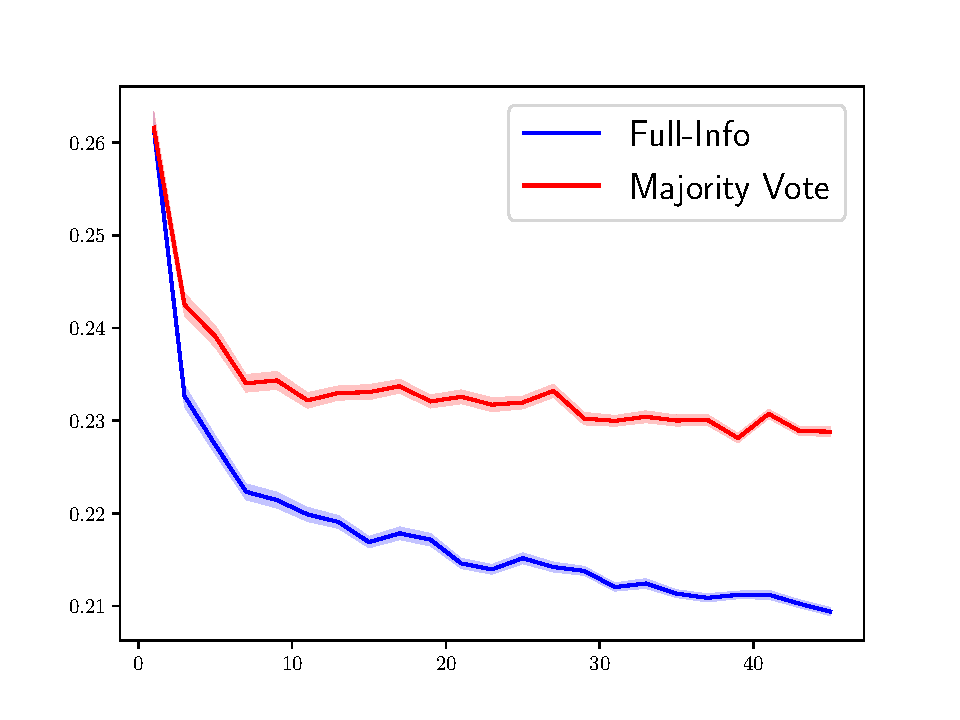
\includegraphics[width=0.45\textwidth]{figure/resnet-class-new.pdf}
			%		& 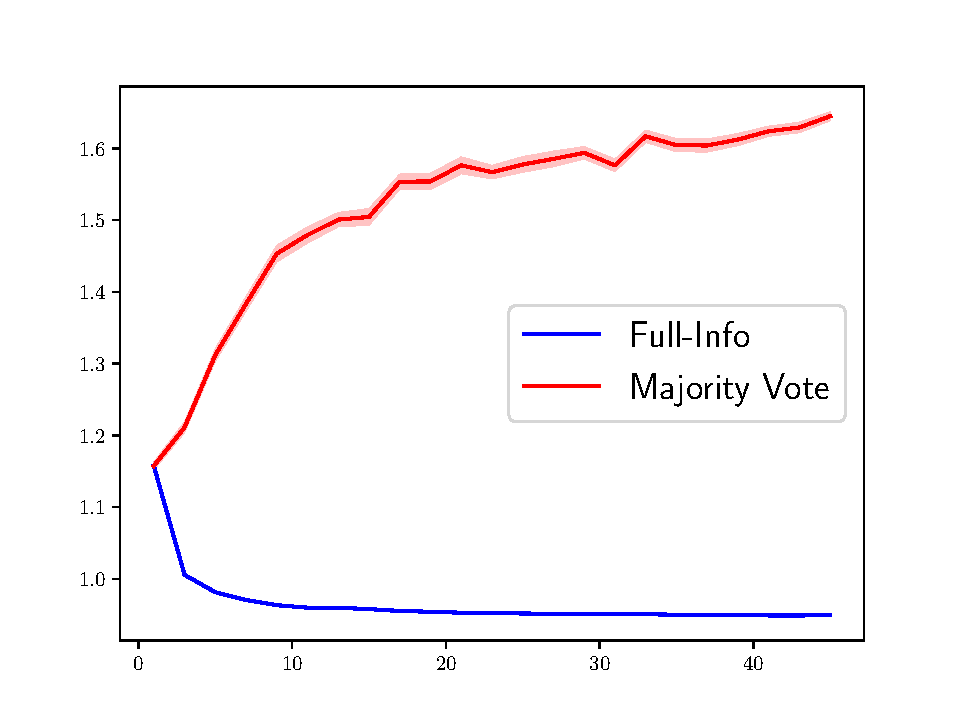
\includegraphics[width=0.45\textwidth]{figure/resnet-calib-new.pdf} \\
			%		(a) & (b) 
			%	\end{tabular}
		%	\caption{Experiments on CIFAR-10H dataset with (a) classification error and (b) calibration error with ResNet features when $d=40$. The classification error is the $0$-$1$ error compared to true labels. The calibration error is measured by $|\mathsf{logit}(\tilde{p}_i) - \mathsf{logit}(\hat{p}_i)|$ where $\tilde{p}_i$ is the predicted probability and $\hat{p}_i$ is the empirical probability. The errors are measured by ten-fold cross-validation. For each fixed $m$, we create $m$ labels for each image by subsampling and average over 100 trials. The error bars show 95\% confidence bands.} \label{fig:cifar}
		%\end{figure}